\begin{figure}[h]
	\centering
	
\includegraphics[scale=2.5]{03_Bedienungsanleitung/img/Logo_HFTl_App.png}
	\label{img:grafik-dummy}
\end{figure}

\begin{center}
	{\huge Benutzerhandbuch}
\end{center}

\begin{center}
	{\huge -  HfTL-APP  -}
\end{center}



\newpage
\subsection{Benutzerhandbuch}
\subsubsection{Funktionsumfang}
In diesem Dokument werden die Benutzerfunktionen der HfTL-APP für
Android-Geräte beschrieben. Es dient als Benutzerhandbuch für die
unterschiedlichen Funktionen der Anwendung und soll Ihnen beim
Ausführen von häufigen Aktionen innerhalb der Anwendung Hilfe bieten.

Die HfTL-APP ist eine mobile Informationslösung für Android Geräte. Die App kann kostenlos über das Rechenzentrum der Hochschule für Kommunikation-Leipzig bezogen werden.

Die HfTL-APP bietet folgende Funktionen:

\begin{itemize}
\item Abfrage der News von der HfTL-Homepage
\item Abfrage der Noten aus QIS/HIS nach erfolgreicher Anmeldung an dem betreffenden System
\item Abfrage des zu einem Studenten passenden Stundenplans
\end{itemize}

\newpage

\subsubsection{Installation}

Vor der Installation müssen auf Ihrem Smartphone APP's mit unbekannter Herkunft freigegeben werden. Dies kann von Smartphone zu Smartphone unterschiedlich sein. In den meisten Fällen ( hier unter Android V5.1 ) findet man den Punkt unter 'Einstellungen/Sicherheit/Unbekannte Herkunft'

\begin{figure}[h]
	\centering
	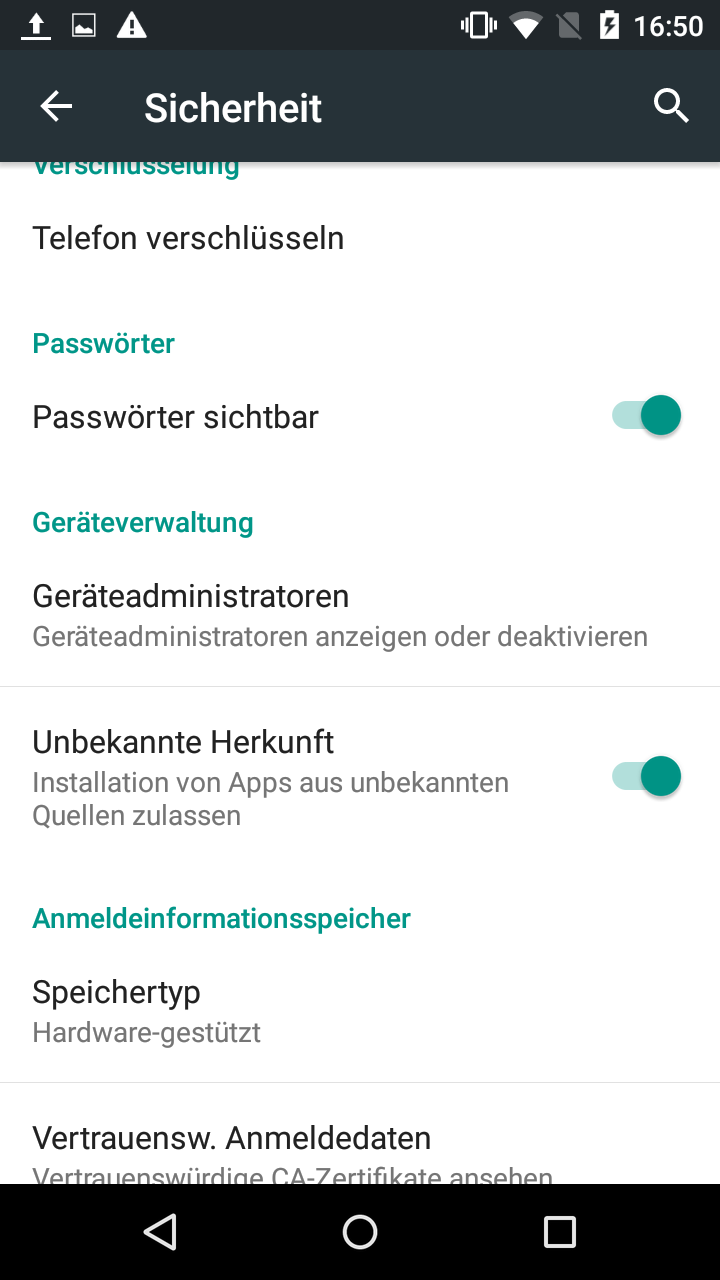
\includegraphics[scale=0.25]{03_Bedienungsanleitung/img/herkunft.png}
	%\caption{eine Grafik ohne Sinn und Verstand}
	%\label{img:grafik-dummy}
\end{figure}

Falls es bei Ihnen anders sein sollte, informieren Sie sich bitte bei Ihrem Handyhersteller dazu.

Um die Installation durchzuführen, laden sie sich bitte die APP von der HFTL-Webseite auf Ihr Android-Smartphone herunter.
Nach Starten der Installation erscheint zunächst die Abfrage der Berechtigungen.

\begin{itemize}
	\item Telefonstatus und Identität abrufen
	\item Ohne das Wissen der Eigentümer Kalendertermine hinzufügen oder ändern und E-Mails an Gäste senden
	\item Netzwerkverbindungen abrufen, Voller Netzwerkzugriff
	\item beim Start ausführen
\end{itemize}

Wenn Sie damit einverstanden sind, bestätigen Sie dieses bitte mit dem Button 'Installieren'


\begin{figure}[h]
	\centering
	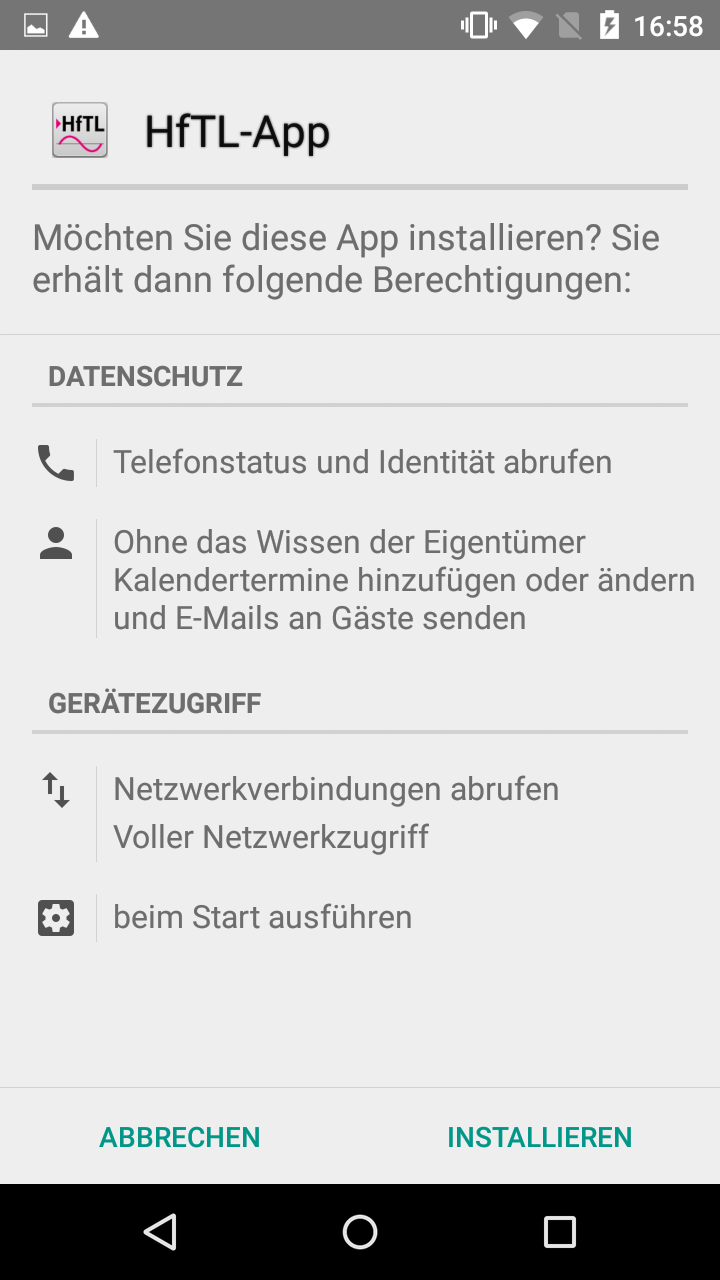
\includegraphics[scale=0.25]{03_Bedienungsanleitung/img/berechtigungen.png}
	%\caption{eine Grafik ohne Sinn und Verstand}
	%\label{img:grafik-dummy}
\end{figure}

Die Installation ist abgeschlossen.

Deinstalliert werden kann die APP wie jede Andere auf Ihrem Smartphone auch.

\newpage

\subsubsection{Startbildschirm}


\begin{figure}[h]
	\centering
	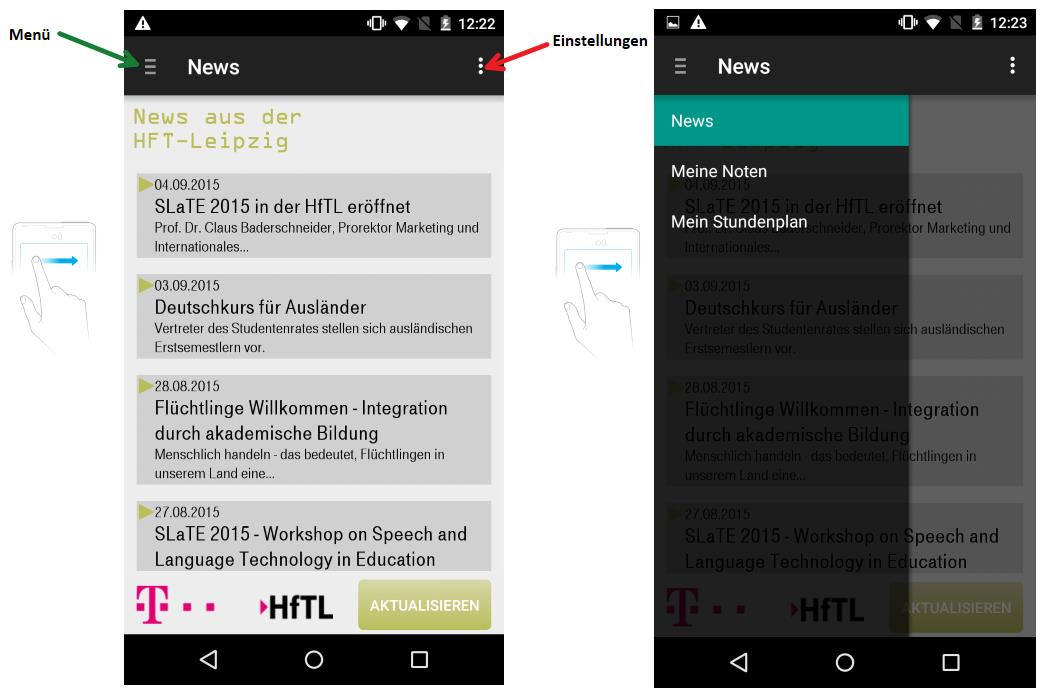
\includegraphics[scale=0.5]{03_Bedienungsanleitung/img/start2.jpg}
	%\caption{eine Grafik ohne Sinn und Verstand}
	\label{img:grafik-dummy}
\end{figure}

%\begin{wrapfigure}{r}{0.5\textwidth}
  %\begin{center}
   % 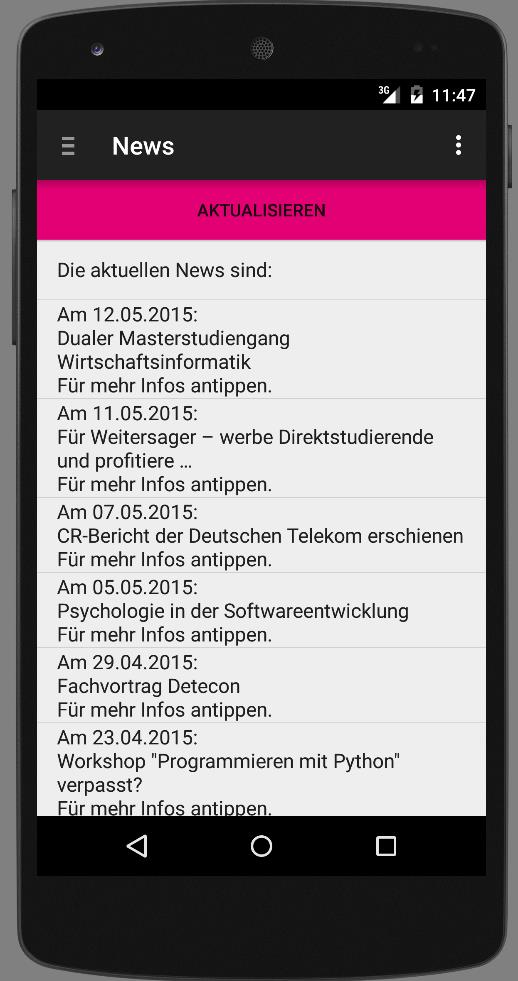
\includegraphics[width=0.5\textwidth]{03_Bedienungsanleitung/img/start.jpg}
  %\end{center}
  %\caption{HFTL-APP©gemeinfrei}
 % \label{reaper}
%\end{wrapfigure}

Nach dem Starten der APP erscheint zunächst die News-Seite. Die News werden bei bestehender Internetverbindung automatisch aktualisiert. Mit klicken auf den Aktualisierungsbutton kann eine manuelle Aktualisierung durch den Nutzer angestoßen werden.

Über den Menü-Button gelangt der Nutzer in das Programm-Menü. Ein Wischen vom linken Bildschirmrand in die Mitte öffnet ebenfalls das Menü. Über den Einstellungs-Button gelangt man in das Einstellungs-Menü. Der Einstellunsgbutton wird nicht bei jedem Gerät gesondert angezeigt. Wenn das Gerät einen Einstellungsbutton unter dem Bildschirm hat z.B. beim Galaxy S3 muss dieser genutzt werden.
Mit Auswählen der einzelnen News gelangt man in deren Detailansicht.


\newpage
\subsubsection{Newsansicht}
\begin{figure}[H]
	\centering
	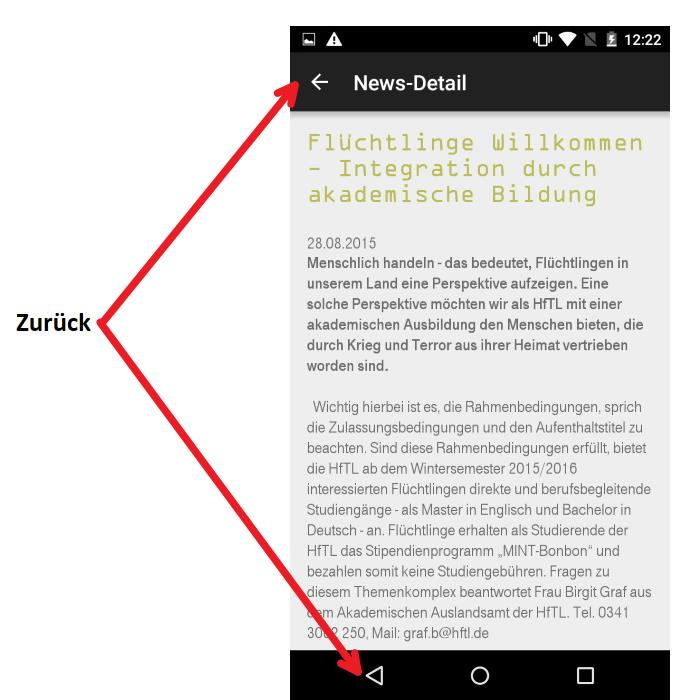
\includegraphics[scale=0.6]{03_Bedienungsanleitung/img/news.jpg}
	%\caption{eine Grafik ohne Sinn und Verstand}
	%\label{img:grafik-dummy}
\end{figure}

Mit den Zurück-Buttons gelangt man in die vorherige Ansicht.



\subsubsection{Noten}

Um die Noten abzurufen geht man zunächst in den Einstellungskontext. Dort kann der Nutzer und das jeweilige Passwort eingegeben werden.
\\
\\
Mit einem Klick auf Benutzername bzw. Passwort öffnet sich ein neuer Kontext, welcher zum eingeben des Benutzernamens bzw. Passwortes auffordert.
\\
\\
Die Eingabe wird mit "'OK"' gespeichert und mit "'Abbrechen"' verworfen. Bei beiden Aktionen schließt sich der Kontext.
Mit Auswählen des Punktes "'Service gestartet"' weist man die APP an, den Service im Hintergrund zu starten. Das Intervall zum Abfragen auf neue Noten kann dann über den Punkt "'Intervall"' ausgewählt werden.

\begin{figure}[h]
	\centering
	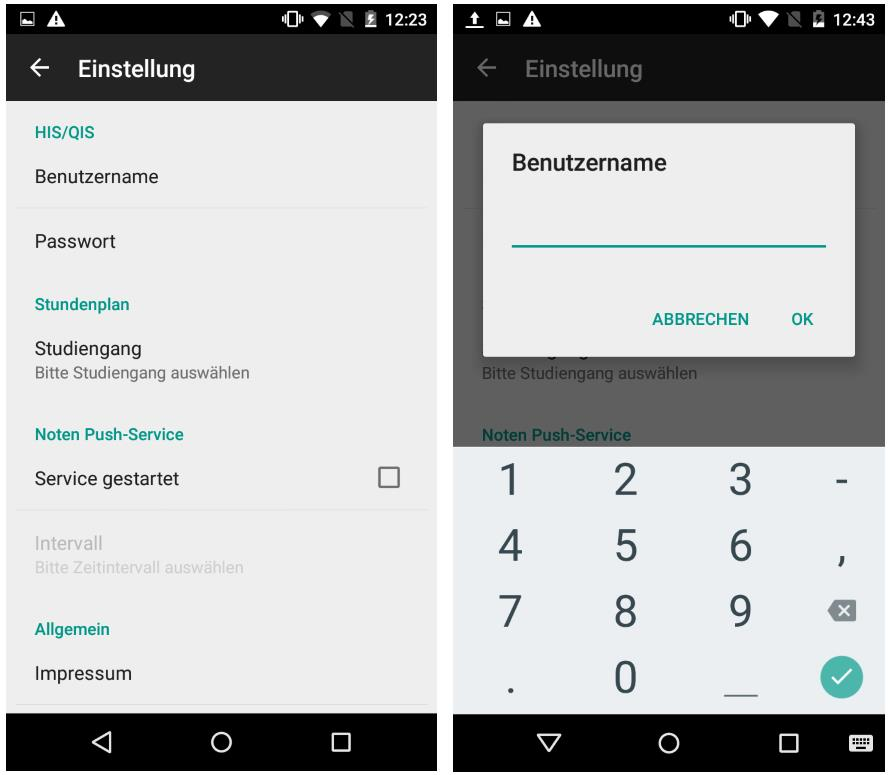
\includegraphics[scale=0.5]{03_Bedienungsanleitung/img/einstellungen.jpg}
	%\caption{eine Grafik ohne Sinn und Verstand}
	%\label{img:grafik-dummy}
\end{figure}


%\begin{figure}[htb]
%    \centering
%    \begin{minipage}{0.45\linewidth}
%        \centering
%        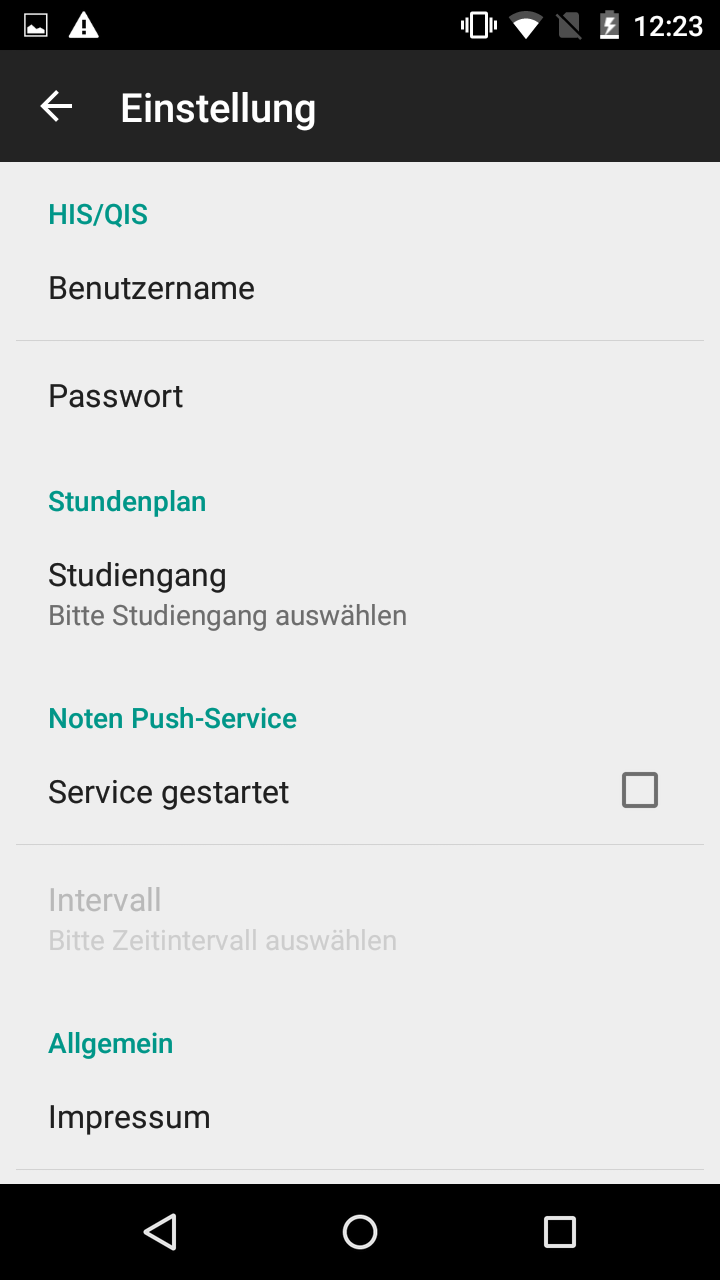
\includegraphics[scale=0.5]{03_Bedienungsanleitung/img/einstellungen.png}
%        %\caption{Beispielbild b}
%    \end{minipage}
%    %\hfill
%    \begin{minipage}{0.45\linewidth}
%        \centering
%        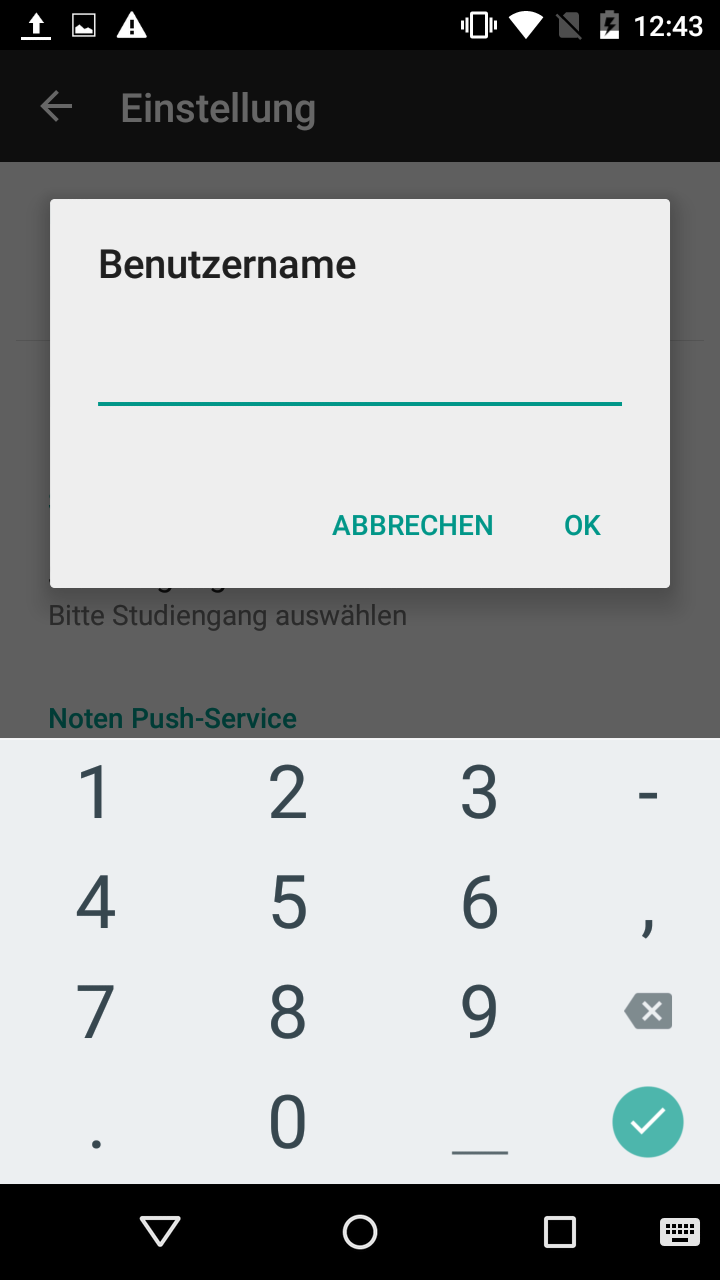
\includegraphics[scale=0.5]{03_Bedienungsanleitung/img/account.png}
%        %\caption{Beispielbild b}
%    \end{minipage}
%\end{figure}


\newpage

Nach erfolgreichem Eintragen des Benutzeraccounts und verlassen der Einstellungen kann über den Menü-Button der Punkt "'Noten"' ausgewählt werden. Hier werden die aktuellen Noten aus QIS/HIS geladen und angezeigt. Sollte es beim Anmelden an QIS/HIS zu einem Fehler kommen, erscheint eine Fehlermeldung und die vorher vorgenommenen Einstellungen sollten noch einmal kontrolliert werden. 

\begin{figure}[H]
	\centering
	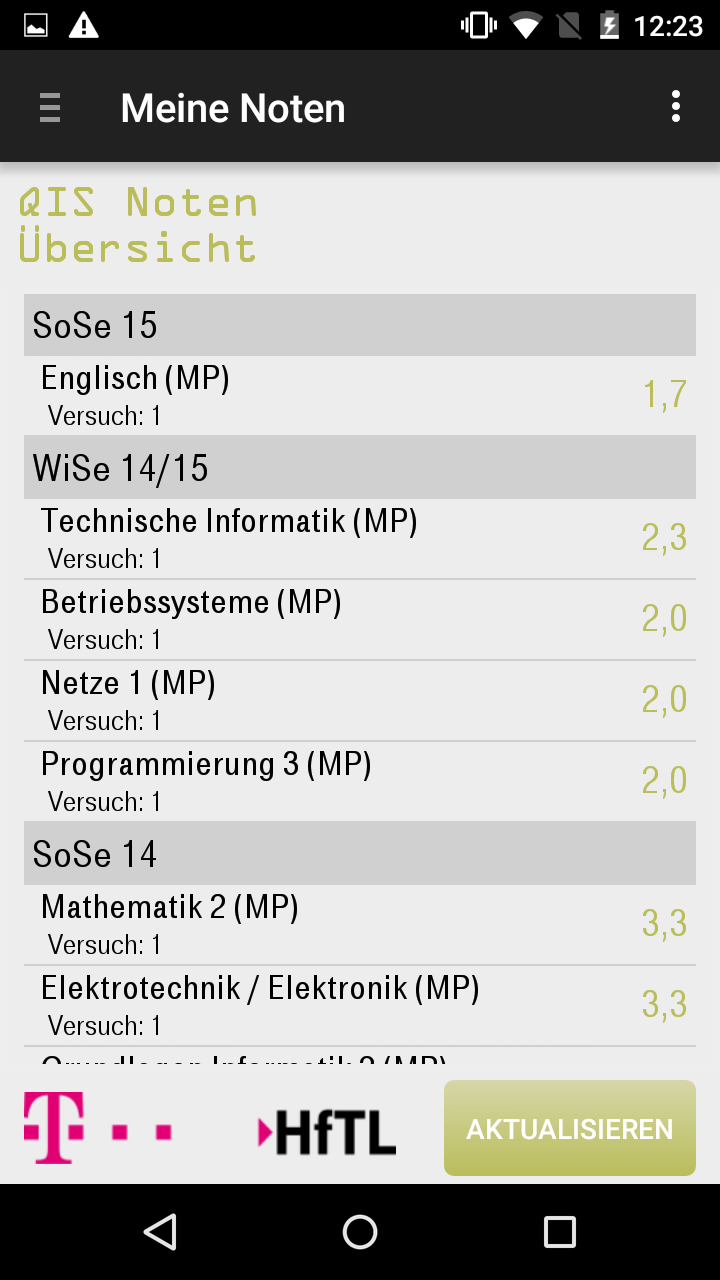
\includegraphics[scale=0.35]{03_Bedienungsanleitung/img/noten.png}
	%\caption{eine Grafik ohne Sinn und Verstand}
	%\label{img:grafik-dummy}
\end{figure}

\newpage

\subsubsection{Stundenplan}

Um sich den jeweiligen Stundenplan anzeigen zu lassen, muss in den Einstellungen unter "'Studiengang"' das korrekte Matrikel ausgewählt werden.
Den Stundenplan erreicht man über das Menü.

\begin{figure}[h]
	\centering
	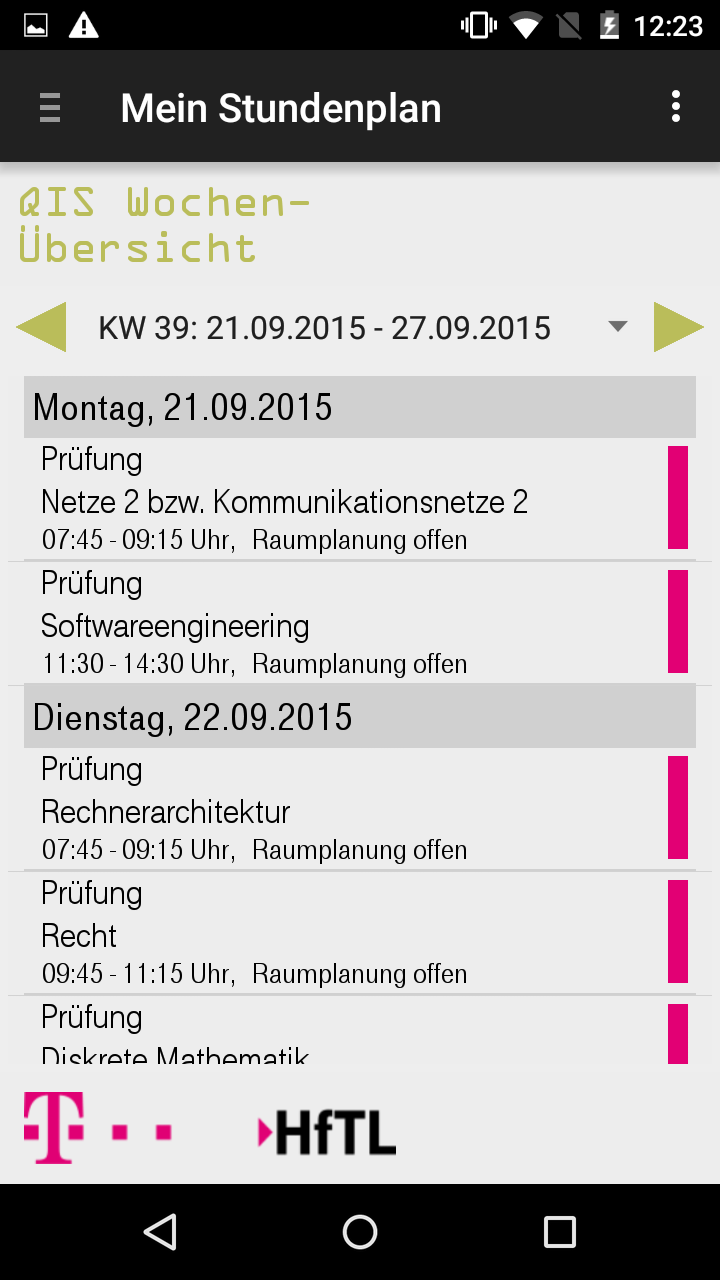
\includegraphics[scale=0.35]{03_Bedienungsanleitung/img/stundenplan.png}
	%\caption{eine Grafik ohne Sinn und Verstand}
	%\label{img:grafik-dummy}
\end{figure}

